\section{Chiral Anomalies}
%
Now we have a chiral gauge theory, SU(2)$_L\otimes$U(1)$_Y$, we can calculate loops! Renormalisation is just as in QCD: in particular the coupling runs (albeit very slowly); $\alpha(0) \approx 1/137$ but $\alpha(m_Z) \approx 1/128$ (determined from precision electroweak measurements at LEP). But when calculating loops we run into problems...
%
\subsection{Triangles (Adler-Bell-Jackiw, 1969)}
%
In QED, all diagrams with an odd number of photons vanish, because $V_\mu \to -V_\mu$ under $C$, as QED is $C$-invariant. Using $V$ to denote a vector vertex $\gamma^\mu$ and $A$ to denote an axial vector vertex $\gamma^\mu \gamma^5$, this means that 
\newline
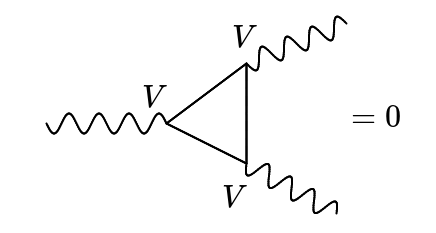
\includegraphics[width=0.4\linewidth]{figs/39a.png}
\newline
but for chiral theories, $C$ is not a symmetry so the triangle graphs are non-zero. The simplest example is the following.
\newline
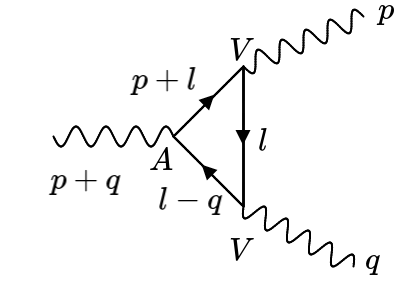
\includegraphics[width=0.4\linewidth]{figs/39b.png}
\newline
Note that this is the same as the crossed version of the graph, because loop momentum $l$ is integrated over. Breaking down the matrix element like
\begin{equation}
\mathcal{M} = \epsilon_\rho(p+q)\epsilon_\mu^*(p)\epsilon_\nu^*(q)\mathcal{M}^{\rho \mu \nu}(p,q),
\end{equation}
we can write
\begin{equation}
\begin{split}
\mathcal{M}^{\rho \mu \nu}(p,q) &= - (-ig)^3)i^3 \int \frac{d^4l}{(2\pi)^4}\ tr \frac{(\gamma^\rho \gamma^5)(\slashed{p} + \slashed{l})\gamma^\mu \slashed{l} \gamma^\nu (\slashed{l} - \slashed{q})}{(p+l)^2l^2(l-q)^2} \\
&= - g^3 \int \frac{d^4l}{(2\pi)^4}\ tr \frac{N^{\rho \mu \nu}}{(p+l)^2l^2(l-q)^2}, 
\end{split}
\end{equation}
where the fermion loop contributes an additional $-$ sign. Note that using $(\gamma^5)^2=1$,
\begin{equation}
N^{\rho \mu \nu} = tr\bigg((\gamma^\rho \gamma^5)(\slashed{p} + \slashed{l})\gamma^\mu \gamma^5 \slashed{l} \gamma^\nu \gamma^5 (\slashed{l} - \slashed{q})\bigg),
\end{equation}
so $AAA=AVV$, but $AAV=VVV=0$, so evaluating $AVV$ is sufficient to cover all cases. 

Considering the relevant Ward identities, conservation of vector current implies $p_\mu \mathcal{M}^{\rho \mu \nu}=0$, $q_\nu \mathcal{M}^{\rho \mu \nu}=0$; and conservation of axial vector current implies $(p+q)_\rho \mathcal{M}^{\rho \mu \nu} = 0$. Let's consider the axial current first:
\begin{equation}
\begin{split}
(p+q)_\rho N^{\rho \mu \nu} &=  tr(\slashed{l}-\slashed{q})(\slashed{p} + \slashed{q})\gamma^5(\slashed{p}+\slashed{l})\gamma^\mu \slashed{l} \gamma^\nu \\
&= tr \gamma^5(\slashed{l}-\slashed{q})(\slashed{p}+\slashed{l}-(\slashed{l}-\slashed{q}))(\slashed{p}+\slashed{l})\gamma^\mu \slashed{l} \gamma^\nu \\
&= tr \gamma^5((\slashed{l}-\slashed{q})(p+l)^2-(\slashed{p}+\slashed{l})(l-q)^2)\gamma^\mu \slashed{l} \gamma^\nu \\
&= 4i\epsilon^{\alpha \mu \beta \nu}((p+l)^2(l-q)_\alpha l_\beta - (l-q)^2(p+l)_\alpha l_\beta) \\
&= +4i\epsilon^{\mu \nu \alpha \beta}((p+l)^2 q_\alpha l_\beta + (l-q)^2 p_\alpha l_\beta),
\end{split}
\end{equation}
so
\begin{equation}
(p+q)_\rho \mathcal{M}^{\rho \mu \nu} = -4ig^3 \epsilon^{\mu \nu \alpha \beta}\int \frac{d^4l}{(2\pi)^4} \bigg[ \frac{q_\alpha l_\beta}{l^2(l-q^2)} + \frac{p_\alpha l_\beta}{l^2(p+l)^2} \bigg].
\end{equation}
The first term in brackets depends only on $q$, so Lorentz invariance implies that $q_\alpha q_\beta \to 0$ because of the $\epsilon^{\mu\nu\alpha\beta}$ factor out the front.  Likewise with the second term and $p$. So $(p+q)_\rho \mathcal{M}^{\rho \mu \nu} = 0$, meaning that the axial current is conserved. 

We also need to check the vector current:
\begin{equation}
\begin{split}
p_\mu N^{\rho \mu \nu} &= tr \gamma^5 (\slashed{p} + \slashed{l})(\slashed{p}+ \slashed{l} - \slashed{l})\slashed{l} \gamma^\nu (\slashed{l} - \slashed{q}) \gamma^\rho \\
&= tr \gamma^5\bigg((p+l)^2\slashed{l} - l^2(\slashed{p}+\slashed{l})\bigg)\gamma^\nu (\slashed{l}-\slashed{q})\gamma^\rho \\ 
&= 4i \epsilon^{\alpha \nu \beta \rho} \bigg((p+l)^2l_\alpha(l-q)_\beta - l^2(p+l)_\alpha(l-q)_\beta \bigg).
\end{split}
\end{equation}
So 
\begin{equation}
\begin{split}
p_\mu \mathcal{M}^{\rho \mu \nu} &= 4ig^3 \epsilon^{\nu \rho \alpha \beta} \int \frac{d^4l}{(2\pi)^4} \bigg[ \frac{l_\alpha(l-q)_\beta}{l^2(l-q^2)} + \frac{(p+l)_\alpha (l-q)_\beta}{(p+l)^2(l-q)^2} \bigg] \\
&= -4ig^3 \epsilon^{\nu \rho \alpha \beta} \int \frac{d^4l}{(2\pi)^4} \bigg[ \frac{l_\alpha q_\beta}{l^2(l-q^2)} - \frac{(p+l)_\alpha (p+q)_\beta}{(p+l)^2(l-q)^2} \bigg],
\end{split}
\end{equation}
where to go from the first line to the second we note that $l-q=p+l-(p+q)$, and consider the antisymmetry of $\epsilon^{\nu\rho\alpha\beta}$. The first term vanishes like before, but the second term depends on both $p$ and $q$.  We can make a shift of the loop momentum (which is integrated over), $l \to l-p$:
\begin{equation}
\frac{(p+l)_\alpha}{(p+l)^2(l+q)^2} \to \frac{l_\alpha}{l^2(l-(p+q)^2)^2},
\end{equation}
so now we see that the second term depends on $(p+q)$ only, so must also vanish. However, the loop integral is linearly divergent, so such a shift is not allowed...

As an aside, consider 
\begin{equation}
\mathcal{I}(a) = \int_{-\infty}^{\infty} dx\ f(x+a).
\end{equation}
If the function is convergent, $\mathcal{I}(a) = \mathcal{I}(0)$. Assume that $f(x) \to c_\pm$ as $x \to \pm \infty$, i.e. that it is linearly divergent. Then
\begin{equation}
\begin{split}
\mathcal{I}(a) - \mathcal{I}(0) &= \int_{-\infty}^{\infty} dx\ \big( f(x+a) - f(x) \big) \\
&= \int_{-\infty}^{\infty} dx\ \big( a f^\prime(x) + \frac{1}{2} a^2 f^{\prime \prime}(x) + ... \big) \\
&= a f^\prime(x)|^{+\infty}_{-\infty} \\
&= a(c_+ - c_-),
\end{split}
\end{equation}
where the $f^{\prime \prime}$ term integrates to 0 because $f^\prime(x) \to 0$ as $x \to \pm \infty$. This works for linearly divergent integrals in four dimensions too: consider
\begin{equation}
\Delta^\alpha(k) = \int \frac{d^4l}{(2 \pi)^4} \big( F^\alpha (l+k) - F^\alpha(l) \big),
\end{equation}
Wick rotate, sending $l \to \tilde{l}$, and Taylor expand:
\begin{equation}
\Delta^\alpha(k) = \int \frac{d^4\tilde{l}}{(2 \pi)^4} \bigg( k^\mu \frac{\partial F^\alpha}{\partial \tilde{l}^\alpha} + ... \bigg).
\end{equation}
Assume at large $\tilde{l}^\mu$ that $F^\alpha(\tilde{l}) \sim A\frac{\tilde{l}^\alpha}{\tilde{l}^4}$, so the integral over $F$ is linearly divergent. Only the first term survives: using the divergence theorem
\begin{equation}
\Delta^\alpha(k) = ik^\mu \int \frac{d^3 S_\mu}{(2\pi)^4} F^\alpha(\tilde{l}),
\end{equation}
where the surface element $d^3 S_\mu = \tilde{l}^2 \tilde{l}_\mu d\Omega_4$, and $d\Omega_4 = 2\pi^2$ is the 4-dimensional solid angle. Expressing $\tilde{l}_\mu \tilde{l}^\alpha \to \frac{1}{4}\delta_\mu^\alpha \tilde{l}^2$,
\begin{equation}
\begin{split}
\Delta^\alpha(k) &= ik^\mu \int \frac{d\Omega_4}{(2\pi)^4} A \frac{\tilde{l}_\mu \tilde{l}^\alpha}{ \tilde{l}^2} \\
&= \frac{i}{32\pi^2} A k^\alpha.
\end{split}
\end{equation}
So shifts in the loop momenta of linearly divergent integrals can give (finite) non-zero terms. Applying this to our integral,
\begin{equation}
\int \frac{d^4l}{(2\pi)^4} \frac{(p+l)_\alpha}{(p+l)^2(l-q)^2} - \int \frac{d^4l}{(2\pi)^4} \frac{l_\alpha}{l^2(l-p-q)^2} = \frac{i}{32\pi^2}p_\alpha \qquad \text{for } A=1,
\end{equation}
so 
\begin{equation}
\begin{split}
p_\mu \mathcal{M}^{\rho \mu \nu} &= -\frac{g^3}{8\pi^2} \epsilon^{\nu \rho \alpha \beta}p_\alpha(p+q)_\beta \\
&= - \frac{g^3}{8 \pi^2} \epsilon^{\nu \rho \alpha \beta}p_\alpha q_\beta \neq 0.
\end{split}
\end{equation}
So the vector current is \textit{not} conserved! This is an anomaly. However, $\mathcal{M}^{\rho \mu \nu}$ clearly depends on how we choose $l$: perhaps there is a better way?

Consider $l^\mu \to l^\mu + k^\mu$ in the integral for $\mathcal{M}^{\rho \mu \nu}$. We end up with
\begin{equation}
\Delta^{\rho \mu \nu} = (-g)^3 ik^\alpha \int \frac{d^3 S_\alpha}{(2\pi)^4} \frac{tr(\gamma^5 \slashed{\tilde{l}}\gamma^\mu \slashed{\tilde{l}}\gamma^\nu \slashed{\tilde{l}}\gamma^\rho)}{\tilde{l}^6},
\end{equation}
and, using $\slashed{\tilde{l}}\gamma^\mu \slashed{\tilde{l}} = -2\tilde{l}^2\gamma^\mu$,
\begin{equation}
\begin{split}
\Delta^{\rho \mu \nu} &= 2ig^3 k^\alpha \int \frac{d\Omega_4}{(2\pi)^4} \tilde{l}^\alpha \frac{4i\epsilon^{\mu \nu \sigma \rho} \tilde{l}_\sigma}{\tilde{l}^2} \\
&= - 8 g^3 k^\alpha \epsilon^{\mu \nu \sigma \rho} \frac{1}{4} \eta_{\alpha \sigma} \frac{\Omega_4}{(2\pi)^4} \\
&= + \frac{g^3}{4\pi^2} \epsilon^{\rho \mu \nu \sigma} k_\sigma.
\end{split}
\end{equation}
So we can shift the anomaly around. Take $k^\mu = \frac{1}{2}(\alpha q^\mu - \beta p^\mu)$: then
\begin{equation}
\begin{split}
p_\mu\mathcal{M}^{\rho \mu \nu} &\to - \frac{g^3}{8\pi^2} \epsilon^{\nu \rho \alpha \beta}p_\alpha q_\beta + \frac{g^3}{4\pi^2} p_\mu\frac{1}{2}(\alpha q_\sigma - \beta p_\sigma) \\
&= -\frac{g^2}{8\pi^2} (1-\alpha) \epsilon^{\nu \rho\alpha \beta}p_\alpha q_\beta, \\
q_\mu\mathcal{M}^{\rho \mu \nu} &\to -\frac{g^2}{8\pi^2} (1-\beta) \epsilon^{\nu \rho\alpha \beta}p_\alpha q_\beta.
\end{split}
\end{equation}
So if we choose $\alpha = \beta = 1$, the vector current is conserved. But watch out:
\begin{equation}
\begin{split}
-(p+q)\mathcal{M}^{\rho \mu \nu} &\to - \frac{g^3}{4\pi^2} \epsilon^{\rho \mu \nu \sigma}(p+q)_\rho \frac{1}{2}(\alpha q_\sigma - \beta p_\sigma) \\
&= -\frac{g^3}{8\pi^2}(\alpha + \beta) \epsilon^{\mu \nu \alpha \beta}p_\alpha q_\beta,
\end{split}
\end{equation}
so now the axial current is anomalous! In other words we can have $\partial^\mu j_\mu = 0$ or $\partial^\mu j_\mu^5 = 0$, but not both. 

So in QED (or QCD), we choose $\partial^\mu j_\mu = 0$ in order that gauge symmetry is exact. But 
\begin{equation}
\partial^\mu j_\mu^5 = - \frac{1}{16 \pi^2} \epsilon^{\mu \nu \alpha \beta} F_{\mu \alpha} F_{\nu \beta} = \frac{1}{8 \pi^2} F_{\mu \nu}^* F^{\mu \nu},
\end{equation}
where $F_{\mu \nu}^* = \frac{1}{2} \epsilon_{\mu \nu \alpha \beta} F^{\alpha \beta}$.
\subsubsection{Notes:}
\begin{enumerate}
\item The right hand side is a topological invariant: the anomaly is not renormalised.
\item The above derivation is regulator-independent. There are problems with $\gamma^5$ in dimensional regularisation and in Pauli-Villars regularisation, but axial symmetry is broken explicitly here.
\item Path integral derivation ????
\item For non-abelian symmetries, there are related anomalies in the box and pentagon diagrams.
\item A practical application is $\pi^0 \to 2\gamma$ (Steinberger, 1951).
\end{enumerate}
%
\subsection{Gauge Anomalies}
%
Consider the left-handed and right-handed currents: $\gamma_5 = P_R - P_L$, $P_R^2=P_R$, $P_L^2=P_L$, $P_RP_L=0$, so $AVV = (R-L)VV = RRR - LLL$. Given that $VVV=0$, $RRR = \frac{1}{2}AVV$ and $LLL = -\frac{1}{2}AVV$.

For $LLL$, we want to have symmetry between each leg of the triangle: choose $1-\alpha$ = $1-\beta$ = $\alpha + \beta$, so $\alpha=\beta=\frac{1}{3}$.
\begin{equation}
\begin{split}
(p+q)_\rho \mathcal{M}_L^{\rho \mu \nu} = - \frac{g^3}{24\pi^2} \epsilon^{\mu \nu \alpha \beta} p_\alpha q_\beta, \\
\text{i.e. } \partial^\mu J_\mu^L = + \frac{1}{96\pi^2}\epsilon^{\mu \nu \alpha \beta}F_{\mu \alpha}^L F_{\nu \beta}^L = - \frac{1}{48 \pi^2}F_{\mu \nu}^{L *} F^{L \mu \nu}.
\end{split}
\end{equation}
So the abelian gauge theory of a single left-handed (or right-handed) chiral fermion is inconsistent: the U(1)$_L$ current is not conserved, so unitarity and renormalisability are spoilt. For consistency, we need $\sum (Q_L^3 - Q_R^3)=0$, e.g. $Q_L=Q_R$ for QED. (There are some weird alternatives possible, such as $Q_L=2$, then 8  with $Q_R=1$.) But what about non-abelian theories, such as SU(2)$_L \otimes$U(1)$_Y$? For a non-abelian gauge theory, there is an additional factor $T_a$ at each vertex.
\begin{figure}[!h]
  \subfloat[]{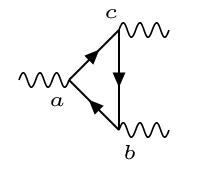
\includegraphics[width=0.3\textwidth]{figs/42a.png}}
 % \hfill
  \subfloat[]{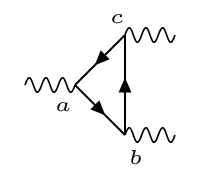
\includegraphics[width=0.3\textwidth]{figs/42b.png}}
\end{figure}
The combination of (a) and (b) gives
\begin{equation}
trT_aT_cT_b + trT_aT_bT_c = trT_a\{T_b,T_c\},
\end{equation}
so for a consistent theory (with no anomaly), we require
\begin{equation}
A_{abc} \equiv trT_a^L\{T_b^L,T_c^L\} - trT_a^R\{T_b^R,T_c^R\} = 0.
\end{equation}
This is automatic for a vector-like theory like QCD, SU(3)$_c$.
%
\subsection{Anomaly Cancellation in the Standard Model (Gross \& Jackiw, 1972)}
%
We require
\begin{equation}
A_{abc} \equiv trT_a^L\{T_b^L,T_c^L\} - trT_a^R\{T_b^R,T_c^R\} = 0
\end{equation}
for $T_a \in$ U(1)$_Y$ or SU(2)$_L$ (both are chiral).
\begin{enumerate}
\item \textbf{SU(2)$_L$:}

$tr \tau_a \{\tau_b, \tau_c \} = 0$ for SU(2), so there is no anomaly. Note that for SU(3)$_L$, $trT_a\{T_b,T_c\}=d_{abc} \neq 0$, so there is no cancellation. In fact SU(N)$_L$ is anomalous for all $N >2$.
\item \textbf{U(1)$_Y$:} 

We need $tr Y_L^3 = tr Y_R^3$.

For leptons, the left-handed leptons have $Y_L = - \frac{1}{2}$, and the right-handed leptons have $Y_e = -1$ and $Y_\nu = 0$. So $tr Y_L^3 = 2 \times (\frac{-1}{2})^3 = -\frac{1}{4}$ (the factor of 2 is because left-handed leptons are in a doublet) and $tr Y_R^3 = (-1)^3 = -1$, so the two don't cancel.

For quarks, left-handed quarks have $Y_Q = \frac{1}{6}$ and right-handed quarks have $Y_u = \frac{2}{3}$ and $Y_d = - \frac{1}{3}$, so $tr Y_L^3 = 2\times 2 \times (\frac{1}{6})^3 = \frac{1}{36}$ (where the factor of 3 comes from the 3 colours). $tr Y_R^3 = = 3 \times ((\frac{2}{3})^3 + (\frac{-1}{3})^3) = \frac{7}{9}$, so again the two don't cancel.

But altogether $-\frac{1}{4} + \frac{1}{36} = -1 + \frac{7}{9}$, so the combination of leptons and quarks cancels! This means that we need three colours of quark in order for the standard model to be consistent. 

\item \textbf{Mixed: }

For SU(N), $tr T_a=0$, so there are no anomalies for $tr T_a Y^2$. But for two SU(N) generators, $tr T_a T_b \propto \delta_{ab}$.
\end{enumerate}